\documentclass[11pt,a4paper]{article}
\usepackage[T1]{fontenc}
\usepackage[utf8]{inputenc}
\usepackage{lmodern}
\usepackage[margin=2.4cm]{geometry}
\usepackage{amsmath,amssymb,amsthm}
\usepackage{booktabs}
\usepackage{graphicx}
\usepackage{xcolor}
\usepackage{microtype}
\usepackage{enumitem}
\usepackage[hidelinks]{hyperref}
\usepackage{url}

\newcommand{\F}{\mathbb{F}}
\newcommand{\Z}{\mathbb{Z}}
\newcommand{\Q}{\mathbb{Q}}
\newcommand{\End}{\operatorname{End}}
\newcommand{\EA}{E_A}
\newcommand{\EC}{E_C}
\newcommand{\ED}{E_D}
\DeclareUrlCommand\art{\urlstyle{tt}}
\makeatletter\g@addto@macro\UrlBreaks{\do\_\do\-\do/}\makeatother
\setlength{\emergencystretch}{3em}
% Hand-written text and the commit; measured tables come from
% numbers_data.tex, generated by figures/make_numbers.py from the records.
% Generated by figures/make_numbers.py from the records; do not edit.
\newcommand{\SummaryRows}{%
L1 & 1 & no & 1341 & 1344 & 1855 & 5 & 0.20 & 1.20 & 128.4 & 64.5\\
L3 & 3 & no & 1991 & 1992 & 2730 & 84 & 1.14 & 5.83 & 192.6 & 96.5\\
L5 & 5 & yes ($\lambda{=}128$) & 2630 & 2632 & 3594 & 51 & 2.30 & 12.78 & 256.8 & 128.5\\
Q3 & 3 & yes & 3904 & 3904 & 5311 & 815 & 5.88 & 37.34 & 384.4 & 192.5\\
Q5 & 5 & yes & 5192 & 5192 & 7050 & --- & --- & --- & 512.7 & 256.5\\}
\newcommand{\ParamRows}{%
L1 & 128 & 1341 & 21 & 1076 & 162 & 256.8 & 144 & 277 & 1344 & 1855 & 1372\\
L3 & 192 & 1991 & 32 & 1594 & 243 & 385.1 & 1059 & 409 & 1992 & 2730 & 2020\\
L5 & 256 & 2630 & 42 & 2106 & 324 & 513.5 & 380 & 536 & 2632 & 3594 & 2660\\
Q3 & 192 & 3904 & 61 & 3125 & 485 & 768.7 & 371 & 791 & 3904 & 5311 & 3932\\
Q5 & 256 & 5192 & 82 & 4155 & 647 & 1025.5 & 975 & 1049 & 5192 & 7050 & 5220\\}
\newcommand{\PerfRows}{%
L1 (jobs=1) & 4.6 [3.6--6.5], $n{=}5$ & 5.4 [4.5--7.5], $n{=}5$ & 0.204 [0.165--0.304], $n{=}50$ & 1.20 [1.08--1.80], $n{=}50$ & 0.208 / 1.25\\
L3 (jobs=1) & 84.1 [76.5--94.0], $n{=}5$ & 87.8 [79.8--97.3], $n{=}5$ & 1.136 [0.796--1.574], $n{=}25$ & 5.83 [5.40--6.30], $n{=}25$ & 1.038 / 6.24\\
L5 (jobs=1) & 50.6 [39.2--80.3], $n{=}5$ & 60.2 [48.6--89.2], $n{=}5$ & 2.301 [1.744--3.063], $n{=}25$ & 12.78 [11.81--14.90], $n{=}25$ & 2.281 / 13.08\\
Q3 (jobs=4) & 815.3 [689.9--940.6], $n{=}2$ & 2592.3 [2395.0--2789.7], $n{=}2$ & 5.880 [5.381--6.562], $n{=}6$ & 37.34 [36.12--38.49], $n{=}6$ & 5.929 / 37.13\\
Q5 (jobs=?) & --- & --- & --- & --- & --- / ---\\}
\newcommand{\OneCoreRows}{%
L1 & 6.5 [4.6--8.5], $n{=}2$ & 0.240 [0.202--0.341], $n{=}10$ & 1.88 [1.78--2.12], $n{=}10$\\
L3 & 85.2, $n{=}1$ & 1.055 [1.044--1.086], $n{=}3$ & 9.61 [9.33--9.65], $n{=}3$\\
L5 & 135.7, $n{=}1$ & 2.938 [2.879--2.992], $n{=}3$ & 22.20 [21.51--25.18], $n{=}3$\\}
\newcommand{\FieldRows}{%
L1 & 21 & 536 & 1674 & 36,539\\
L3 & 32 & 1760 & 5479 & 59,891\\
L5 & 42 & 2957 & 9019 & 88,919\\
Q3 & 61 & 5936 & 18343 & 152,385\\
Q5 & 82 & 10656 & 32345 & 240,125\\}
\newcommand{\ChainRows}{%
L1 & 569 & 0.63 & 1122 & 670\\
L3 & 828 & 2.99 & 3640 & 664\\
L5 & 1091 & 6.45 & 5922 & 657\\
Q3 & 1598 & 18.69 & 11697 & 638\\}
\newcommand{\BenchRunId}{%
run-20261017T2022Z-kem-bench}
\newcommand{\DecLOne}{%
1.2}
\newcommand{\EncLOne}{%
0.20}
\newcommand{\KgQThree}{%
14\,min}
\newcommand{\StepMults}{%
583--720}
\newcommand{\StepFactor}{%
2.3--2.8}

\newcommand{\EigenxCommit}{d89d790}
\newcommand{\MethodText}{%
One campaign, run \art{\BenchRunId}, measured every operation on one host: a
shared cloud VM with 4 vCPUs (Intel Xeon at 2.10\,GHz, one thread per core),
Linux 6.18, rustc~1.97.0, release profile, \art{eigenx} commit
\art{\EigenxCommit}. Isolation is the lowest level (L0): no core pinning
for the all-core rows, and \texttt{taskset -c 0} for the single-core rows.
Other tenants' load is not controlled. The harness is
\art{eigenx:examples/bench_kem.rs}.
\begin{itemize}[nosep]
\item For each set it draws several fresh keys. Key generation is timed in
  wall time and in process CPU time, because it is a rejection search: a
  single sample says little, and parallel attempts (\texttt{jobs}) trade
  CPU time for wall time.
\item Under each key it runs encapsulation then decapsulation of an honest
  ciphertext several times, one PKE round trip of a 1\,KiB message with
  associated data, and one public-key degree test, the attacker's oracle
  (\S\ref{sec:security}). Every result is checked.
\item In the same binary it times $\F_p$ and $\F_{p^2}$ arithmetic.
\end{itemize}
Samples per set: L1 5 keys $\times$ 10, L3 and L5 5 $\times$ 5, Q3 2
$\times$ 3, Q5 1 $\times$ 3, and single-core L1 2 $\times$ 5, L3 and L5 1
$\times$ 3. The Q sets use \texttt{jobs}=4 for key generation; every other
row uses \texttt{jobs}=1. Medians are reported with the range, because the
samples are few and the host is noisy.}


\title{Eigen-S\'eta: performance and security white paper\\[0.3em]
\large Measured cost of every operation at every parameter set, security
levels, known attacks, risks and open questions}
\author{Anonymous}
\date{2026-10-17 --- research document, not peer reviewed}

\begin{document}
\maketitle

\begin{abstract}
Eigen-S\'eta~v2 is an isogeny-based key encapsulation mechanism whose
trapdoor is a secret endomorphism of the public curve. This white paper
gives the measured cost of key generation, encapsulation, decapsulation and
authenticated public-key encryption on all five parameter sets of the
maintained Rust implementation, all measured on one host in one campaign.
It then states the security level of each set in the two metrics that
matter for NIST's categories, catalogues every attack we know, and ranks
the risks and open questions. The specification, proofs and full analysis
are in the companion paper~\cite{EigenSetaPaper}. The short version is as
follows.
\begin{itemize}[nosep]
\item Public keys and ciphertexts are 1.3--5.2\,kB. A shared secret is
  32~bytes.
\item On a shared 4-vCPU cloud VM, L1 decapsulates in about \DecLOne\,s and
  encapsulates in \EncLOne\,s. Key generation is a rejection search, from
  seconds at L1 to \KgQThree\ at Q3. Q5 key generation took \KgQFive\ with four workers.
\item Against every NIST post-quantum KEM measured on the same host,
  Eigen-S\'eta is slower by orders of magnitude. At level~1 it decapsulates
  about \RatioDecLOne\ times slower than ML-KEM and 2,600--7,600 times
  slower than BIKE, FrodoKEM and Classic McEliece. Its 1.3\,kB keys and
  ciphertexts are competitive.
\item L1, L3 and L5 meet NIST categories 1, 3 and 5 only in NIST's gate
  count under MAXDEPTH. At least $2^\lambda$ quantum queries is met only by
  L5 (at $\lambda=128$), Q3 and Q5.
\item The largest risk is the hidden orientation of the public curve. If it
  became effective, it would give subexponential quantum key recovery at
  every set.
\end{itemize}
Security is a conjecture. No one outside the project has analysed the
scheme. Do not use it to protect data.
\end{abstract}

\tableofcontents

%------------------------------------------------------------------
\section{Summary}\label{sec:summary}

Table~\ref{tab:summary} is the one-page answer. Every number is measured in
run \texttt{\BenchRunId} (\S\ref{sec:perf}) or derived by the cost model
(\S\ref{sec:security}). The record of each value is named in the section
that discusses it.

\begin{table}[h]
\centering
\caption{The five parameter sets at a glance. Sizes are exact. Times are
medians on one shared 4-vCPU VM (\S\ref{sec:method}). Security columns are
$\log_2$ of the cheapest known attack, from the cost model.}
\label{tab:summary}
\resizebox{\textwidth}{!}{%
\begin{tabular}{lllrrrrrrrr}
\toprule
set & NIST cat. (gates) & $\ge2^\lambda$ queries & $\log_2p$ & pk = ct (B) & sk (B) & keygen (s) & encaps (s) & decaps (s) & classical & quantum queries\\
\midrule
\SummaryRows
\bottomrule
\end{tabular}}
\end{table}

Recommended use, if the conjectures hold: L5, Q3 and Q5 for post-quantum
deployments; L1 and L3 only where security against classical attack and
NIST's gate-count metric are enough.

%------------------------------------------------------------------
\section{The scheme in one page}\label{sec:scheme}

Let $\ED$ be the curve with complex multiplication by $\Z[(1+\sqrt{-7})/2]$
($j=-3375$) over $\F_p$, with $p=2^{E+1}3^Fc-1$. Write $\omega$ for its
endomorphism of degree~2, and $(P_D,Q_D)$ for an eigenbasis of $\omega$ on
$\ED[2^E]$.

\paragraph{Key generation.} Draw a secret odd degree $f$ from an interval of
about $2^{2\lambda+20}$ values. Find $\alpha\in\End(\ED)$ of norm
$f(2^E-f)$ with Cornacchia. Split the Kani isogeny with kernel
$\{([f]R,\alpha R)\}$ to obtain $\varepsilon:\ED\to\EA$ of degree~$f$. The
public key is $\EA$ with $x$-coordinates of $\lambda_1\varepsilon(P_D)$,
$\lambda_2\varepsilon(Q_D)$ and their difference. These points are
eigenvectors of the hidden endomorphism $\tau=\varepsilon\omega\hat\varepsilon$.
The secret key is a function of $f$ alone.

\paragraph{Encapsulation.} Pick $s$ modulo $d=3^F$. Walk the $3^F$-isogeny
$\varphi$ with kernel $P_3+sQ_3$ to $\EC$. Push the public basis through it
and mask the images by $(a,b)=G(s,H(pk))$. The ciphertext is $\EC$ and three
$x$-coordinates. The key is $H_K(s,ct)$, under the Fujisaki--Okamoto
transform with implicit rejection.

\paragraph{Decapsulation.} The masks act diagonally on eigenvectors, so the
holder of $f$ knows the action of the trace-zero endomorphism
$\psi=2\varphi\tau\hat\varphi-tdf$ on the masked points. One
$(2^E,2^E)$-isogeny in dimension two (Kani's lemma, theta coordinates)
evaluates $\psi$ on $\EC[3^F]$. Its kernel gives $\hat\varphi$ and hence
$s$. The decapsulator then re-encrypts and compares.

\paragraph{Why it is secure, if it is.} Without $f$, the public key is an
isogeny of unknown degree $f$ from a known curve, and the ciphertext is a
FESTA-type masked-torsion instance~\cite{BMP23}. The Castryck--Vercauteren
observation~\cite{CV23}, that an eigenbasis of a \emph{known} endomorphism
defeats diagonal masks, is the trapdoor. Hiding the endomorphism's degree
is what is supposed to deny it to everyone else.

Figure~\ref{fig:map} shows the objects and the attack routes of
\S\ref{sec:attacks}.

\begin{figure}[h]
\centering
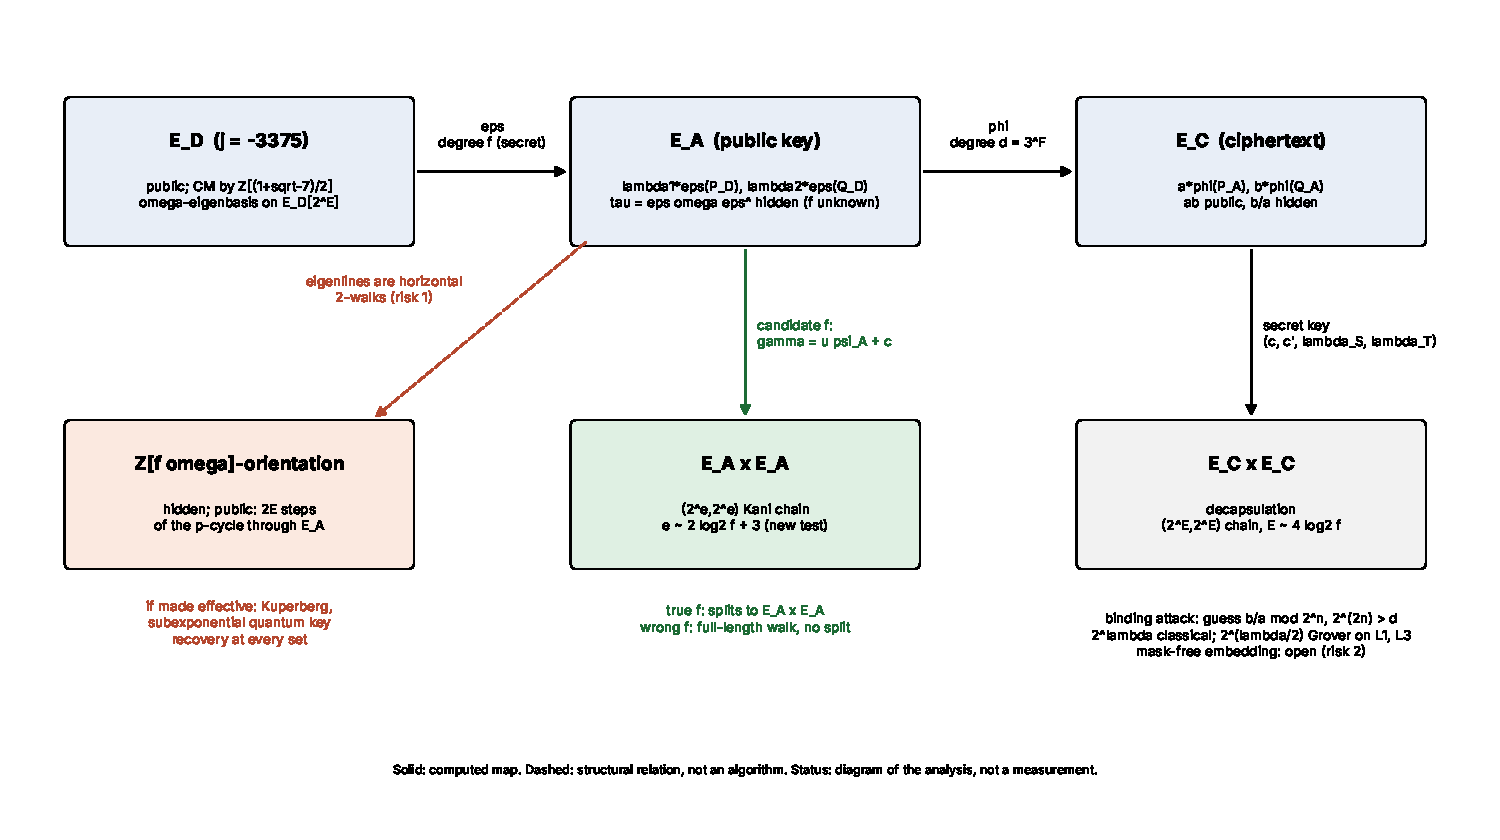
\includegraphics[width=\textwidth]{figures/attack_map.pdf}
\caption{Objects of the scheme and the attack routes considered. Diagram of
the analysis, not a measurement.}
\label{fig:map}
\end{figure}

%------------------------------------------------------------------
\section{Parameter sets and sizes}\label{sec:params}

The primes come from a deterministic public search~\cite{EigenX}. Fix
$\lambda$ and set $m=2$ for the L sets or $m=4$ for the Q sets. Then
$F=\lceil m\lambda/\log_23\rceil$, $E$ is the smallest exponent with
$2^E>28d^2f_{\max}^2$, and $c$ is the smallest cofactor for which $p$ is
prime under fixed-base Miller--Rabin and $p\equiv3,5,6\pmod 7$. At
$\lambda=128$ and $m=4$ the search reproduces the L5 prime, so L5 is also
the quantum-hardened level-1 set.

\begin{table}[h]
\centering
\caption{Parameters and object sizes in bytes. Public key and ciphertext are
four $\F_{p^2}$ elements each. Files add an 8-byte header. A PKE ciphertext
is the KEM ciphertext, a 12-byte nonce, the message and a 16-byte tag.
Sizes measured by the benchmark (\texttt{sizes} rows); parameters from
\texttt{eigenx:src/params\_generated.rs}.}
\label{tab:params}
\resizebox{\textwidth}{!}{%
\begin{tabular}{lrrrrrrrrrrr}
\toprule
set & $\lambda$ & $\log_2p$ & limbs & $E$ & $F$ & $\log_2 d$ & $c$ & $f$ bits & pk = ct & sk & PKE overhead\\
\midrule
\ParamRows
\bottomrule
\end{tabular}}
\end{table}

The prime grows as $p\approx d^5$, about $10.5\lambda$ bits for the L sets.
The reason is that one Kani chain must decode an endomorphism of degree
$7d^2f^2$. Two half-chains would cut this to about $d^3$
(\S\ref{sec:open}). That is the single largest efficiency lever.

%------------------------------------------------------------------
\section{Performance}\label{sec:perf}

\subsection{Method}\label{sec:method}
\MethodText

\subsection{Results}

\begin{table}[h]
\centering
\caption{Wall time in seconds, median [min--max] over $n$ samples, all
four vCPUs available (the KEM uses scoped threads inside decapsulation and
encapsulation). Key generation is one attempt loop per key
(\texttt{jobs}=1 for L, \texttt{jobs}=4 for Q). Every decapsulation and PKE
decryption returned the right value. Run \texttt{\BenchRunId}.}
\label{tab:perf}
\resizebox{\textwidth}{!}{%
\begin{tabular}{lrrrrr}
\toprule
set & keygen wall & keygen CPU & encaps & decaps & PKE enc / dec (1\,KiB)\\
\midrule
\PerfRows
\bottomrule
\end{tabular}}
\end{table}

\begin{table}[h]
\centering
\caption{The same operations restricted to one core (\texttt{taskset -c 0}).
Median [min--max]. Run \texttt{\BenchRunId}.}
\label{tab:onecore}
\begin{tabular}{lrrr}
\toprule
set & keygen & encaps & decaps\\
\midrule
\OneCoreRows
\bottomrule
\end{tabular}
\end{table}

\begin{figure}[h]
\centering
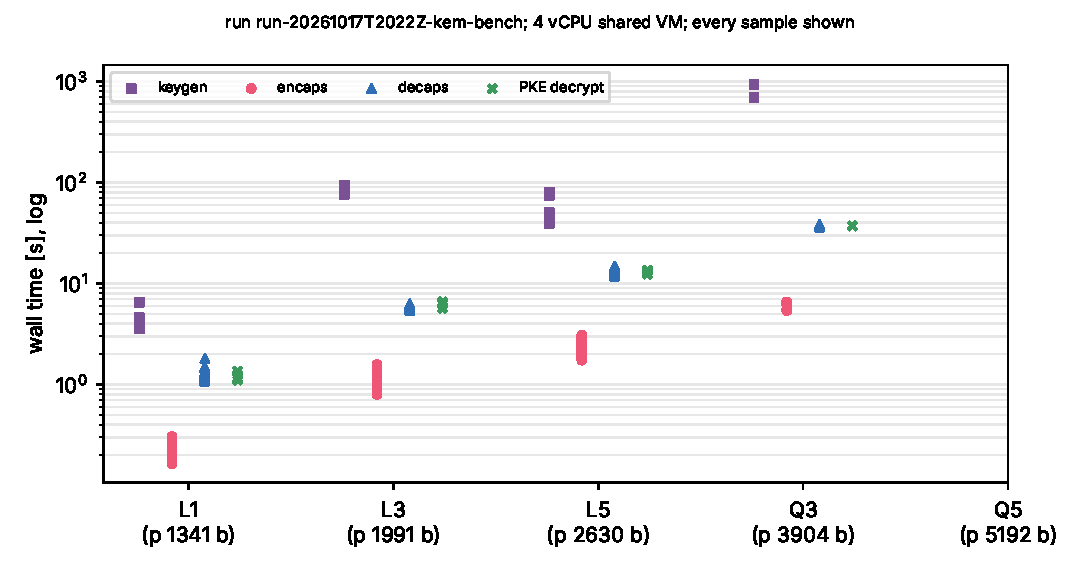
\includegraphics[width=\textwidth]{figures/perf.pdf}
\caption{Every sample of every operation, log scale, all cores. Measured;
run \texttt{\BenchRunId}.}
\label{fig:perf}
\end{figure}

\begin{table}[h]
\centering
\caption{Field arithmetic in the same binary: $\F_p$ and $\F_{p^2}$
multiplication (best of 15 loops of 20,000) and $\F_p$ inversion (mean of
200). Measured, ns.}
\label{tab:field}
\begin{tabular}{lrrrr}
\toprule
set & limbs & $\F_p$ mul & $\F_{p^2}$ mul & $\F_p$ inversion\\
\midrule
\FieldRows
\bottomrule
\end{tabular}
\end{table}

\PerfDiscussion


%------------------------------------------------------------------
\section{How far off: comparison with other post-quantum KEMs}\label{sec:compare}

\subsection{Same host}
Table~\ref{tab:compare} runs every post-quantum KEM that NIST standardised
or shortlisted on the benchmark host, through liboqs~0.13.0 (the \art{oqs}
Rust crate~0.11.0). Each operation is timed individually on one pinned core,
until 2\,s or 1,000 operations. The table shows the mean of the medians of
two repetitions. Record:
\art{crypto:research/eigen_seta_whitepaper_20261017/records/pqkem_same_host/}.
liboqs was built as a distribution build, so it picks its AVX2 or AVX-512
code at run time on this CPU. The one exception is HQC: liboqs ships only
PQClean's portable implementation for it, so the HQC rows understate an
optimised HQC. The Eigen-S\'eta rows are the all-core medians of
Table~\ref{tab:perf}. An earlier measurement of ML-KEM-512 with the
portable RustCrypto crate (no AVX2), taken while Q5 key generation loaded the
host, gave 37 and 47\,$\mu$s for encapsulation and decapsulation
(\art{records/mlkem_same_host/}). It is kept as a record but not used in
the table. Eigen-S\'eta's decapsulation uses up to four threads, while
liboqs uses one, which flatters Eigen-S\'eta by up to about 1.7 times
(Table~\ref{tab:onecore}).

\begin{table}[h]
\centering
\caption{Post-quantum KEMs on one host. Median wall time per operation;
sizes in bytes (k = thousand). Every decapsulation was checked.
$^\dagger$Portable reference implementation (no AVX2).}
\label{tab:compare}
\begin{tabular}{lrrrrr}
\toprule
KEM & keygen & encaps & decaps & pk & ct\\
\midrule
\CompareRows
\bottomrule
\end{tabular}
\end{table}

\begin{figure}[h]
\centering
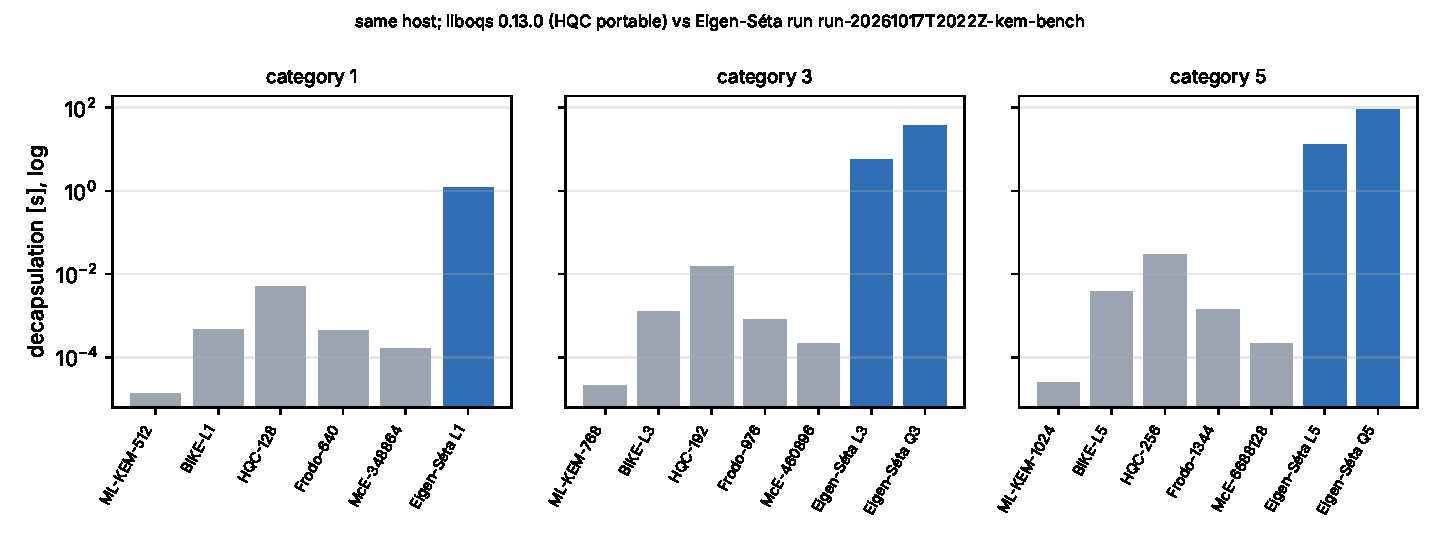
\includegraphics[width=\textwidth]{figures/compare.pdf}
\caption{Decapsulation time on the benchmark host, log scale, by NIST
category. Grey: liboqs 0.13.0 (HQC portable). Blue: Eigen-S\'eta. Measured.}
\label{fig:compare}
\end{figure}

\paragraph{What the table says.}
\begin{itemize}[nosep]
\item \emph{Against ML-KEM, the standard,} Eigen-S\'eta L1 is about
  \RatioEncLOne\ times slower to encapsulate and \RatioDecLOne\ times slower
  to decapsulate. By set, the decapsulation ratio is \RatioDecAll. That
  runs from four orders of magnitude at L1 encapsulation to six and a half
  at Q5 decapsulation.
\item \emph{Against the code-based and conservative lattice KEMs:} at
  level~1, BIKE, FrodoKEM and Classic McEliece decapsulate 2,600 to 7,600
  times faster than Eigen-S\'eta L1. Even the portable HQC is about 230
  times faster. Classic McEliece's key generation, the slowest in the
  field at 40\,ms to 0.3\,s, is still 100 to 200 times faster than ours.
\item \emph{Where Eigen-S\'eta is competitive: size.} At level~1 its
  1,344-byte key and ciphertext are close to ML-KEM and BIKE, smaller than
  HQC and FrodoKEM, and 190 times smaller than a Classic McEliece public
  key. The quantum-hardened sets lose much of that edge (3.9--5.2\,kB).
\end{itemize}

\subsection{Other isogeny schemes (published figures)}
No other isogeny encryption scheme is available in a library we could run.
Their published figures are on other hardware: PIKE in C on an Intel i7 at
2.3\,GHz encrypts in 23\,ms and decrypts in 15\,ms at NIST level~I~\cite{PIKE}.
POKÉ's SageMath proof of concept takes about 100\,ms for each, with a
431-bit prime, a 324-byte public key and a 648-byte ciphertext~\cite{POKE}.
FESTA's SageMath implementation on an Apple M1 Pro takes 3.09\,s to encrypt
and 9.14\,s to decrypt, with a 1292-bit prime and 561 and 1,122-byte key and
ciphertext~\cite{BMP23}. One constant-time CSIDH-512 group action is about
125\,Mcycles on Skylake~\cite{CTIDH}. Against PIKE, Eigen-S\'eta L1 decrypts
about 80 times slower and encrypts about 9 times slower. The main reason is
the prime: about $10\lambda/3$ bits for POKÉ and PIKE against $10.5\lambda$
here.

\subsection{What would close the gap}
Two half-chains would bring the prime to about $d^3$, roughly 800 bits at L1
(\S\ref{sec:open}). Field arithmetic was portable Rust and can be improved (it since has
been: aburan28/eigenx\#6). The theta step itself is already at the cost of
its formulas, so the chain gains little from step-level work. Our estimate for all of this together is about one order of
magnitude. That would put Eigen-S\'eta level with POKÉ and PIKE, and still
three to four orders of magnitude behind ML-KEM and the code-based KEMs at
decapsulation.

%------------------------------------------------------------------
\section{Security level}\label{sec:security}

\subsection{How the levels are computed}
The levels are \emph{derived}, not measured: no attack in
Table~\ref{tab:attacks} can be run at real size. They come from the cost
model in \art{eigenx:src/security.rs}, run by
\art{eigenx:examples/security_estimate.rs} (record
\art{crypto:research/eigen_seta_whitepaper_20261017/records/security_estimate.txt}).
For each attack the model gives three numbers: classical operations, quantum
oracle queries, and quantum gates under NIST's MAXDEPTH. The gate count uses
the parallel-Grover accounting: a search over $2^n$ items with an oracle of
$2^g$ gates and depth $2^{g-4}$ costs $2^{n/2+g}$ gates if serial Grover fits
the depth limit, and $2^{n+(g-4)+g-\mathrm{MAXDEPTH}}$ otherwise. The model
favours the attacker in that it ignores memory and uses $p^{1/3}$ for path
finding. The tables in this section charge $2^8$ $\F_{p^2}$ multiplications
of Karatsuba cost per $(2,2)$-step, which the next paragraph corrects to
$2^{7.5}$.

\paragraph{What we measured, and a correction.} One input of the model can
be checked: the cost of an isogeny-chain step, the Grover oracle's inner
loop. Table~\ref{tab:chain} times the attacker's public-key degree test and
divides by its length $e$ and by the $\F_{p^2}$ multiplication time, giving
\StepMults\ ``multiplication-equivalents'' per step. That figure is not a
step cost. It includes the work before the chain (about half of the test,
mostly ladders) and every field addition. An earlier version of this
section read it as showing that the model's $2^8$ errs on the attacker's
side. That reading was wrong.

Exact operation counts settle it (\art{eigenx:examples/chain_opcount.rs},
feature \texttt{opcount}; aburan28/eigenx\#7). A theta $(2,2)$-step of the
same test costs 566.6 $\F_p$ products, which is 188.9 $\F_{p^2}$
multiplications, or $2^{7.56}$. The model's $2^8$ therefore overcharged the
attacker. eigenx\#7 lowers the constant to $2^{7.5}$, the measured cost
rounded down. That lowers every quantum-gate column of the mask-guess and
degree-search rows by 1.0 bit at MAXDEPTH $2^{40}$ and $2^{64}$, and by
0.5 bit at $2^{96}$. The classical and quantum-query floors are unchanged.
Table~\ref{tab:attacks} and Fig.~\ref{fig:margins} still show the $2^8$
model; with the correction the L1 gate floor is $2^{150.2}/2^{126.2}/2^{97.1}$
against AES-128's $2^{130}/2^{106}/2^{74}$. Tier~A still holds for L1, L3
and L5, with margins of about 20 bits.

\begin{table}[h]
\centering
\caption{Measured cost of the attacker's chain step: one public-key degree
test of length $e$ for the true $f$ of each key (accepted in every case).
``Mult.-equiv.'' is wall time per step divided by $\F_{p^2}$ multiplication
time; it includes setup and additions, so it is not a step cost (see text). Median over keys. Run \texttt{\BenchRunId}.}
\label{tab:chain}
\begin{tabular}{lrrrr}
\toprule
set & $e$ & time per test (s) & $\mu$s per step & mult.-equiv. per step\\
\midrule
\ChainRows
\bottomrule
\end{tabular}
\end{table}

\subsection{Levels per set}

\begin{table}[h]
\centering
\caption{Cost of each attack, $\log_2$ (derived). Chains for the
degree search are the public-key test of \S\ref{sec:attacks}. The
hidden-orientation row is a lower bound under the false assumption that the
class-group action can be evaluated, not an attack.}
\label{tab:attacks}
\resizebox{\textwidth}{!}{%
\begin{tabular}{llrrrrr}
\toprule
target & attack & L1 & L3 & L5 & Q3 & Q5\\
\midrule
key & degree search, classical (chains) & 265.5 & 396.9 & 523.5 & 777.9 & 1035.5\\
key & degree search, Grover (queries) & 132.7 & 198.4 & 261.7 & 389.0 & 517.8\\
key & $\End(\EA)$, classical $p^{1/3}$ & 447.0 & 663.7 & 876.7 & 1301.3 & 1730.7\\
key & $\End(\EA)$, quantum $p^{1/4}$ & 335.2 & 497.8 & 657.5 & 976.0 & 1298.0\\
key & hidden orientation, $f^{1/2}$ (lower bound) & 138.5 & 204.5 & 268.0 & 395.5 & 524.5\\
message & mask guess $+$ Kani, classical & 129.0 & 193.0 & 257.0 & 385.0 & 513.0\\
message & mask guess $+$ Kani, Grover (queries) & 64.5 & 96.5 & 128.5 & 192.5 & 256.5\\
message & claw on $\varphi$, classical $\sqrt d$ & 128.4 & 192.6 & 256.8 & 384.4 & 512.7\\
message & claw on $\varphi$, quantum $d^{1/3}$ & 85.6 & 128.4 & 171.2 & 256.2 & 341.8\\
\midrule
\multicolumn{2}{l}{classical floor} & 128.4 & 192.6 & 256.8 & 384.4 & 512.7\\
\multicolumn{2}{l}{quantum-query floor} & 64.5 & 96.5 & 128.5 & 192.5 & 256.5\\
\multicolumn{2}{l}{gate floor, MAXDEPTH $2^{40}/2^{64}/2^{96}$} & 151/127/98 & 218/194/162 & 284/260/228 & 415/391/359 & 545/521/489\\
\multicolumn{2}{l}{AES reference (NIST)} & 130/106/74 & 193/169/137 & 258/234/202 & 193/169/137 & 258/234/202\\
\bottomrule
\end{tabular}}
\end{table}

\begin{figure}[h]
\centering
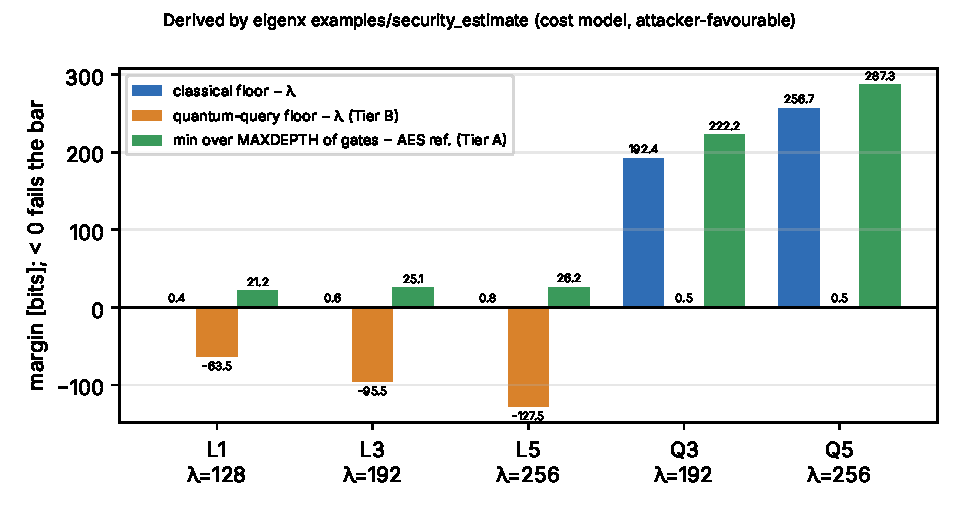
\includegraphics[width=0.85\textwidth]{figures/attack_margins.pdf}
\caption{Margin of each set over its target in each metric (derived). A
negative bar fails that bar.}
\label{fig:margins}
\end{figure}

\subsection{What this means for NIST categories}

\begin{description}[style=nextline]
\item[Tier A: gate count under MAXDEPTH (NIST's stated metric).] L1, L3 and
  L5 clear the AES-128, -192 and -256 references at all three depth limits.
  Under the corrected $2^{7.5}$ step cost, the margins at the tightest limit
  are about 20.2, 24 and 25 bits; the table and figure retain the original
  $2^8$ model. In this metric they are \emph{conjectured} to be categories
  1, 3 and 5.
\item[Tier B: at least $2^\lambda$ quantum queries against every known attack.]
  The binding attack on the L sets, Grover over the mask ratio, needs only
  $2^{\lambda/2}$ queries. That is $2^{64.5}$ at L1 and $2^{96.5}$ at L3,
  the same exposure as FESTA. Only L5 (at $\lambda=128$), Q3 and Q5 meet
  this bar. Recommending L1 or L3 as quantum-hardened would be false.
\item[Classical.] Every set has a classical floor of at least $2^\lambda$.
  For the Q sets it is about $2^{2\lambda}$.
\end{description}
Both tiers assume the hidden orientation stays ineffective (\S\ref{sec:risks}).

%------------------------------------------------------------------
\section{Attacks}\label{sec:attacks}

This is every attack we know, with its status. Costs are in
Table~\ref{tab:attacks}. ``Measured'' means we ran the attack or its
oracle. ``Derived'' means it was computed from the parameters.

\subsection{Key recovery}
\begin{description}[style=nextline]
\item[The secret key is a function of $f$ (measured).] Given $f$, a working
  key follows in polynomial time. The Kani scalars come from one
  sum-of-two-squares, and the eigenvalue scaling is irrelevant. So key
  recovery means finding $f$. The test was run on real keys
  (\art{eigenx:src/cryptanalysis/degree.rs}).
\item[Degree search with the public-key test (measured; new).] Guess $f$
  and test it with a Kani chain of length $e\approx2\log_2f$ on
  $\EA\times\EA$ for $\gamma=u\psi_A+c$, where $\psi_A=2\tau-tf$ has degree
  $7f^2$. The test needs no ciphertext and is about half a decapsulation. A
  wrong guess is rejected only at the final split. Near misses that agree
  with $f$ on many low bits fare no better, so there is no bit-by-bit
  recovery. In the 2026-10-17 assessment, 158 wrong candidates across L1,
  L3 and L5 were all rejected and the true degree was always
  accepted~\cite{EigenSetaPaper}. The search space is about $2^{2\lambda+10}$
  admissible degrees, so this is not binding.
\item[Generic endomorphism ring or path finding (derived).] $\varepsilon$
  is with overwhelming probability the unique shortest isogeny from $\ED$
  to $\EA$. So any connecting path yields $f$ after lattice reduction. The
  cost is $p^{1/2}$ classically, or $p^{1/3+o(1)}$ heuristically with large
  memory~\cite{Wes26}, and $p^{1/4}$ quantumly. Since $p\approx2^{10.5\lambda}$
  this is never close.
\item[Meet in the middle on $\varepsilon$ (derived).] This needs $f$ to be
  smooth and its factorisation known. It costs at least $\sqrt f$, about
  $2^{\lambda+10}$.
\item[SIDH torsion attacks on the public key (derived).] The public key
  gives $\varepsilon$ on $\ED[2^E]$ up to a diagonal matrix, with
  $2^E\gg f^2$. The Castryck--Decru, Maino--Martindale et al.\ and Robert
  attacks~\cite{CD23,MMPPW23,Rob23} need the degree. With $f$ hidden they
  reduce to the degree search. Hiding the degree is the countermeasure, as
  in terSIDH and binSIDH~\cite{BF23}.
\item[Hidden orientation (derived; the main risk).] $\EA$ is oriented by
  $\Z[f\omega]$, and the public eigenlines are horizontal $2$-walks of
  length $E$ in that orientation. With an effective orientation, the
  class-group action could be evaluated. Kuperberg's sieve would then
  recover the key in subexponential quantum time~\cite{Wes21orient}, and
  one endomorphism would give $\End(\EA)$ in $|7f^2|^{1/4}$ classical
  time~\cite{HLMW23}. No algorithm we know makes it effective
  (\S\ref{sec:risks}).
\item[Self-pairings (derived: not applicable).] These need
  $m^2\mid\mathrm{disc}$ for accessible $m$~\cite{CHMMvBV23}. The
  discriminant $-7f^2$ is odd and prime to 3.
\item[The earlier public-degree variant (measured: broken).] The toy
  prototype's ``walk'' variant used a public degree $5^k$. Its key is a
  function of $k$, and it was broken on 5 of 5 ciphertexts. Version~2
  exists to fix this.
\end{description}

\subsection{Message recovery}
\begin{description}[style=nextline]
\item[Mask guessing plus a torsion attack (derived; binding).] The pairing
  reveals the product of the masks but not their ratio. Guessing the ratio
  modulo $2^n$ with $2^{2n}>d$ gives the torsion data for Robert's attack.
  The cost is $\sqrt d\approx2^\lambda$ classically and $d^{1/4}$ Grover
  queries. This is FESTA's estimate~\cite{BMP23} and the binding attack on
  every set.
\item[Claw finding on the sender's isogeny (derived).] This costs $\sqrt d$
  classically and $d^{1/3}$ with Tani's algorithm. Tani is no better than
  classical van Oorschot--Wiener once memory is costed~\cite{JS19}. A
  meet-in-the-middle is implemented in \art{eigenx:src/cryptanalysis/mitm3.rs}.
\item[Lollipop attacks (derived: not applicable as stated).] The attacks of
  Castryck and Vercauteren on FESTA and M-SIDH~\cite{CV23} need a known
  low-degree endomorphism with the public basis as eigenbasis. The only such
  endomorphisms are in $\Z[\tau]$, which has degree at least $2f^2$ and is
  unknown without $f$. No element of $\Z[\tau]$ has an eigenline on the
  $3^F$-torsion, because $3$ is inert in $\Q(\sqrt{-7})$.
\end{description}

\subsection{Chosen-ciphertext, implementation and physical attacks}
\begin{description}[style=nextline]
\item[Adaptive and decryption-failure attacks (derived).] FO with implicit
  rejection answers every malformed ciphertext with a pseudorandom key. The
  adaptive FESTA attacks~\cite{MO23} need a validation or timing oracle,
  which constant-time decapsulation removes. No honest decapsulation has
  failed in any recorded run. That is evidence, not a proof that the
  correctness error is zero.
\item[Timing (partly measured).] The secret phase of decapsulation was
  shown instruction-count constant on the earlier Mumford build. It has not
  been re-measured on the theta build. Key generation is variable time by
  design.
\item[Side channels beyond timing (open).] Leaking $\alpha$ or $f$ through
  power or EM reduces the scheme to a subexponential quantum problem.
  Masks are per ciphertext, so the mask-leakage results~\cite{DIKM25} apply
  as to FESTA. Fault attacks on torsion masking~\cite{GLM26} also apply, and
  the FO check is the only countermeasure.
\end{description}


%------------------------------------------------------------------
\section{Risks, big unknowns and open questions}\label{sec:risks}


Ranked by how much would fall if each went wrong.
\begin{enumerate}[label=\textbf{R\arabic*.}]
\item \emph{The hidden orientation becomes effective.} The public key is a
  segment of a horizontal $2$-walk in the hidden $\Z[f\omega]$-orientation.
  Turning that into an evaluable class-group action, for example with the
  level-structure frameworks~\cite{DFP24,Arpin24} or sesquilinear pairings,
  gives subexponential quantum key recovery at \emph{every} set. Larger
  parameters do not help, because the Q sets enlarge $d$ and not $f$.
  Nobody has tried. \textbf{This is the big unknown.}
\item \emph{A mask-free higher-dimensional embedding.} The subgroups
  $\varphi\langle P_A\rangle$ and $\varphi\langle Q_A\rangle$ and the mask
  product are public. A dimension-4 or -8 Kani embedding from these alone
  would remove the $\sqrt d$ search behind every security level. This is
  open and not ruled out.
\item \emph{The eigenbasis gives a handle on $f$.} The attacker knows
  $\tau$ on $\EA[2^E]$ up to the scalar $f$. We found no use for this
  beyond guessing $f$ whole, and the public-key test needs all of $f$. A
  partial-information attack would break key recovery.
\item \emph{The decisional assumption.} IND-CPA needs a decisional problem.
  Every basis is an eigenbasis of some endomorphism, so the assumption is
  about the size of the smallest diagonal one. It has no argument beyond
  the absence of a distinguisher.
\item \emph{Correctness error.} The FO bound has a term $q_D\delta$. We have
  observed $\delta=0$ in every run but have no proof for the fixed chain
  schedule.
\item \emph{The Grover-oracle constant.} The gate-count tier rests on an
  oracle cost model. Its chain-step constant now matches our exact count,
  rounded down (\S\ref{sec:security}); it was $2^8$, which overcharged the
  attacker by 0.5--1.0 bit in gates. It has had no external review. Tier~B
  does not depend on it.
\item \emph{Implementation.} Constant-time behaviour has not been
  re-verified on the theta build. Key generation is variable time. There is
  no second implementation and no independent check of the known-answer
  tests.
\end{enumerate}


\subsection{Open questions}\label{sec:open}

\begin{enumerate}[label=\textbf{Q\arabic*.}]
\item Can the two public $2$-walks, possibly with level structure or a
  sesquilinear pairing, make the $\Z[f\omega]$-orientation of $\EA$
  effective? (R1)
\item Can a Kani embedding of dimension 4 or 8 be built from the masked
  subgroups and $ab$ alone, without guessing the ratio? (R2)
\item Is there a test that rejects a wrong degree using less than all of
  $f$, for example modulo $2^j$ through a smaller endomorphism? (R3)
\item Is decisional eigen-CIST well posed, and is there a distinguisher on
  the size of the smallest diagonal endomorphism? (R4)
\item Can the correctness error be proved zero for every admissible key?
  (R5)
\item Engineering: decrypt with two half-chains to bring $p$ from about $d^5$
  to $d^3$, and add compressed keys and ciphertexts and constant-time key
  generation.
\end{enumerate}


%------------------------------------------------------------------
\section{Implementation status}\label{sec:impl}

\begin{itemize}
\item Rust crate in the sibling repository \art{eigenx}: constant-time
  $\F_p$ arithmetic (Montgomery-friendly reduction, safegcd inversion),
  x-only ladders, 3-isogeny chains, and a theta-coordinate $(2,2)$-chain
  for decapsulation. It has a CLI with a versioned file format,
  known-answer tests, hostile-input tests and CI.
\item The cost model (\art{src/security.rs}) and runnable attack components
  (\art{src/cryptanalysis/}) are in the same crate.
\item A NIST package draft (\art{docs/nist/}) states what is still missing:
  an external review of the FO proof, a proof of zero correctness error,
  constant-time evidence on the current source, a C reference
  implementation, NIST-DRBG KATs, and timings on the reference platform.
\end{itemize}


%------------------------------------------------------------------
\section{Reproduction}\label{sec:repro}

\begin{itemize}
\item Benchmark: \art{cargo run --release --example bench_kem -- <set> <keys> <trials> <jobs>}
  at \art{eigenx} commit \texttt{\EigenxCommit}. Records, host description,
  graphs and the run report are in
  \art{crypto:research/eigen_seta_whitepaper_20261017/}, with copies in
  \art{crypto:benchmarks/20261017-eigen-seta-whitepaper/}.
\item Security levels: \art{cargo run --release --example security_estimate}.
\item Specification, proofs and the full analysis: the companion
  paper~\cite{EigenSetaPaper}, \art{crypto:papers/eigen-seta/}.
\end{itemize}


\bibliographystyle{alpha}
\bibliography{refs}
\end{document}
